\documentclass[journal]{IEEEtran}
\usepackage{graphicx}
\usepackage{cite}
\usepackage{multirow}
\usepackage{booktabs}
\usepackage{siunitx}
\usepackage[T1]{fontenc}
\usepackage[pdftex,breaklinks,pdfauthor={MSD Team P17101},pdfcreator={Philip Linden},pdftitle={P17101 Arcjet Thruster}]{hyperref}
\usepackage{nomencl}
\usepackage{chngcntr}
\makenomenclature{}

% cite.sty was written by Donald Arseneau
% V1.6 and later of IEEEtran pre-defines the format of the cite.sty package
% \cite{} output to follow that of IEEE. Loading the cite package will
% result in citation numbers being automatically sorted and properly
% "compressed/ranged". e.g., [1], [9], [2], [7], [5], [6] without using
% cite.sty will become [1], [2], [5]--[7], [9] using cite.sty. cite.sty's
% \cite will automatically add leading space, if needed. Use cite.sty's
% noadjust option (cite.sty V3.8 and later) if you want to turn this off.
% cite.sty is already installed on most LaTeX systems. Be sure and use
% version 4.0 (2003-05-27) and later if using hyperref.sty. cite.sty does
% not currently provide for hyperlinked citations.
% The latest version can be obtained at:
% http://www.ctan.org/tex-archive/macros/latex/contrib/cite/
% The documentation is contained in the cite.sty file itself.

% http://edge.rit.edu/edge/P17101/public/Home

\title{P17101: Design and Characterization of a 1kW Arcjet Thruster}
\author{
  Philip~Linden$^{*}$\thanks{$^{*}$MEng Student, Department of Mechanical Engineering},
  James~Gandek$^{\dagger}$\thanks{$^{\dagger}$BS Student, Department of Mechanical Engineering},
  Dylan~Bruce$^{\dagger}$,
  Matt~Giuffre$^{\dagger}$,
  Anthony~Higgins$^{\ddagger}$\thanks{$^{\ddagger}$BS Student, Department of Electrical Engineering},
  David~Yin$^{\ddagger\S}$\thanks{$^{\S}$Only contributed to MSD I}
}
  % page header for pages other than cover page
  \markboth{P17101 Arcjet Thruster}%
  {Linden \MakeLowercase{\textit{et al.}}: Multidisciplinary Senior Design, RIT}

\begin{document}
\maketitle
% correct bad hyphenation here
\hyphenation{explor-ation explor-atory}

\begin{abstract}
An arcjet electrothermal propulsion system was developed to RIT Space Exploration (SPEX). The arcjet thruster demonstrates the degree of practicality in implementing electrothermal propulsion systems. The arcjet assembly generates an electrical arc across the thruster nozzle's throat, ionizing nitrogen propellant in order to achieve a greater specific impulse compared to cold gas propulsion.
\end{abstract}

\label{sec:nomenclature}
% List all symbols and subscripts used for any math equations.
% This will add the units
%----------------------------------------------
\newcommand{\nomunit}[1]{%
\renewcommand{\nomentryend}{\hspace*{\fill}#1}}
%----------------------------------------------
% gas dynamics
\nomenclature{$A$}{Cross-sectional area of nozzle
  \nomunit{\,\si{\meter\squared}}}
\nomenclature{$p$}{Gas pressure
  \nomunit{\,\si{\kilo\pascal}}}
\nomenclature{$v$}{Gas flow velocity
  \nomunit{\,\si{\meter\per\second}}}
\nomenclature{$\dot{m}$}{Gas mass flow rate
  \nomunit{\,\si{\kilo\gram\per\second}}}
\nomenclature{$\alpha$}{Diverging nozzle half-angle
  \nomunit{\,\si{\deg}}}
% rocket equations
\nomenclature{$F$}{Thrust
  \nomunit{\,\si{\newton}}}
\nomenclature{$I_{sp}$}{Specific impulse
  \nomunit{\,\si{\second}}}
\nomenclature{$g_0$}{Standard acceleration due to gravity
  \nomunit{\,\SI{9.81}{\meter\per\second\squared}}}
\printnomenclature{}

\section{Introduction}
\label{sec:intro}
\IEEEPARstart{R}{IT} Space Exploration (SPEX) provided a use-case scenario to serve as the basis for this exploration into satellite propulsion.
The mission objective is to design a communicaitons satellite that is capable of maintaining a polar geostationary orbit for 10 years.

In practice, satellites in Earth orbit for long-duration missions (5--25 years) encounter perturbations to their trajectories over time from residual atmospheric and orbital particles, or from variations in Earth's gravity field.
These spacecraft perform short station-keeping maneuvers periodically to compensate for drift and orbital decay.

An electrothermal rocket engine is method of propulsion by which a pressurized inert gas stored at ambient temperature (cold gas) is released and heated electrically before being expelled out of a nozzle.
Two proven methods of electrothermal propulsion are \emph{resistojets}, which use conventional heat exchangers to heat the propellant, and \emph{arcjets}, which pass the propellant through an electrical arc to heat the gas.

Electrothermal propulsion is advantageous over conventional chemical or cold-gas rockets for use by long-life satellites since the engines may be small in size, have no moving parts, and are more efficient at the expense of thrust.
While resistojets and arcjets require more elecrical power than chemical rockets, for example, the electrical energy may be recovered over time by photovoltaic panels whereas propellant fuel is a finite resource for these spacecraft.

A tabletop prototype thruster was designed and tested to explore the feasibility of this type of system with less strict requirements compared to the limitations of building a flight-worthy system.
A tabletop version does not require integration with a spacecraft, and mass and spatial limitations are relaxed.

\section{Design Theory}
\label{sec:method}
% Describe why an arcjet was selected over a resistojet.
In low power (\SI{1}{\kilo\watt}) applications, an arcjet offers up to 200\% gains in efficiency over a resistojet thruster~\cite{sutton2010rocket}.
\autoref{fig:power-vs-isp} identifies the typical use cases and performance characteristics of arcjets compared to various other types of electrothermal thrusters.
Arcjets achieve a greater specific impulse compared to resistojets but produce less thrust.
Thus a maneuver would take a longer amount of time using an arcjet but would consume less propellant overall for the same maneuver as compared to a resistojet.
\begin{figure}[htp]
  \centering
  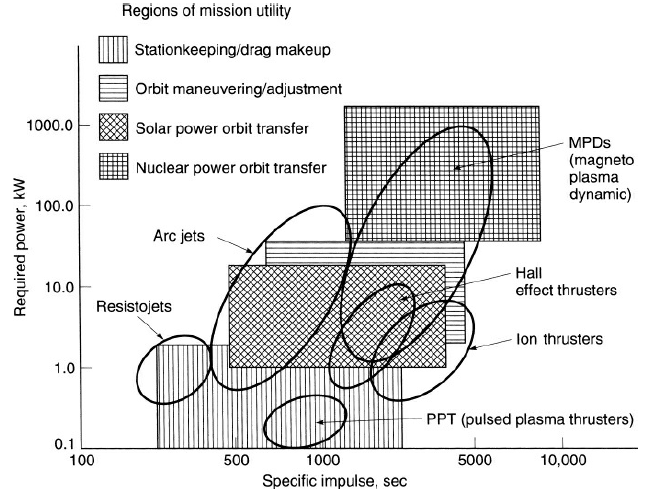
\includegraphics[width=\linewidth]{figs/power-vs-isp_sutton}
  \caption[Types of electrothermal propulsion]{There are various types of electrothermal propulsion with respect to typical performance and mission utility.
  In the \SI{1}{\kilo\watt} range, arcjets typically have a higher specific impulse than resistojets. (Sutton~2010)
\label{fig:power-vs-isp}}
\end{figure}

% Justify propellant selection (and explain paschen curve?)
The ideal propellant for arcjet engines is one which can be stored for long periods of time, has a low atomic mass, and favorable thermodynamic conditions during heating and expansion.
NASA identifies Hydrogen (H$_{2}$), Ammonia (NH$_{3}$), and Hydrazine (N$_{2}$H$_{3}$) as ideal propellants for arcjets~\cite{nasa1992considerations}.
Unfortunately, these gases are toxic or difficult to handle on a university campus.
Nitrogen (N$_{2}$) is an easy-to-handle alternative that has relatively favorable ionization and thermodynamic characteristics, and has been used in similar low-power arcjet demonstrations~\cite{olin2012report,olin2012sim}.
% High level gas dynamics analysis
\begin{figure}[htp]
  \centering
  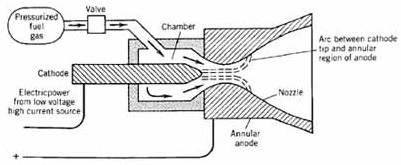
\includegraphics[width=\linewidth]{figs/cross-section_nasa}
  \caption[Arcjet cross-section]{A cross sectional view of a typical arcjet shows the expected flowpath of propellant and the expected region of the electric current arc. The propellant is ionized and heated by the arc then expanded through the nozzle. (NASA~GRC~1992)
\label{fig:x-section-nasa}
}
\end{figure}

Gas enters the chamber and is ionized and heated by a high-current arc that extends from the cathode to the throat of the anodic nozzle to form a plasma.
The plasma reaches sonic speed in the throat and is supersonically accelerated as it expands through the nozzle.

Thrust is a function of the momentum of the flow exiting the nozzle.
\begin{equation}
\label{eq:thrust}
  F=\dot{m}v_e + (p_e-p_b)A_e
\end{equation}
 Where $F$ is thrust, $\dot{m}$ is mass flow rate of propellant, $v$ is flow velocity, $A$ is nozzle cross sectional area of the nozzle, and subscript $e$ denotes parameters at the nozzle exit while $p_b$ denotes atmospheric backpressure.
 In space, $p_b$ is negligible and the thruster is design around such condition.

 A thruster's efficiency is described in terms of specific impulse, $I_{sp}$, which may be used to compare performance with other space propulsion methods.
 \begin{equation}
 \label{eq:isp}
   I_{sp}=\frac{F}{\dot{m} g_0}
 \end{equation}
% some calculations?
In the ideal condition using gaseous N$_2$ as propellant, a conical nozzle with $\alpha=15$ is capable of \SI{0}{\newton} of thrust without a sustained arc.
At sea-level, \SI{0}{\newton} of thrust is expected.
\textbf{Include theoretical calcs for cold thrust to compare performance with theory in order to validate design.
Also predict thrust with arc on.
Show Isp predictions for given thrust values and estimated mass flow rates.}

\begin{table}[hbp]
  \caption{Theoretical thrust and Isp values with respect to space and sea-level operation, total pressure $p_0= $\SI{137.9}{\kilo\pascal}.
\label{tab:theoretical-performance}
}
  \begin{tabular}{lrrrrr}
    \toprule
    & & \multicolumn{2}{c}{Without arc} & \multicolumn{2}{c}{With arc} \\
    & $p_b$ (\si{\kilo\pascal}) & Thrust (\si{\newton}) & $I_{sp}$ (\si{\second}) & Thrust (\si{\newton}) & $I_{sp}$ (\si{\second}) \\
    \midrule
    Vacuum & $0$ & $0$ & $0$ & $0$ & $0$ \\
    Sea-level & $101.3$ & $0$ & $0$ & $0$ & $0$  \\
    \bottomrule
  \end{tabular}
\end{table}

\section{System Overview}
% outline the main system architecture.
\subsection{Thruster}
% Describe the main components of the thruster and how they interact. Be sure to include material selection justifications. Show some basic analysis and predictions for performance with justification.
Propellant flows into a stainless steel body and is spun into a vortex about the tip of the cathode, where it passes through an electric arc before being accelerated through a conical nozzle.
The flow swirler doubles as a high-temperature ceramic insulator.
The insulator and cathode are mounted concentrically into a low-temperature PTFE thermal and electrical insulator, which is fixed to the thruster test stand.
The nozzle is electrically insulated from the steel body by a non-conductive ceramic spacer.
% how much energy transferred from arc to plasma?
\begin{figure}[htp]
  \centering
  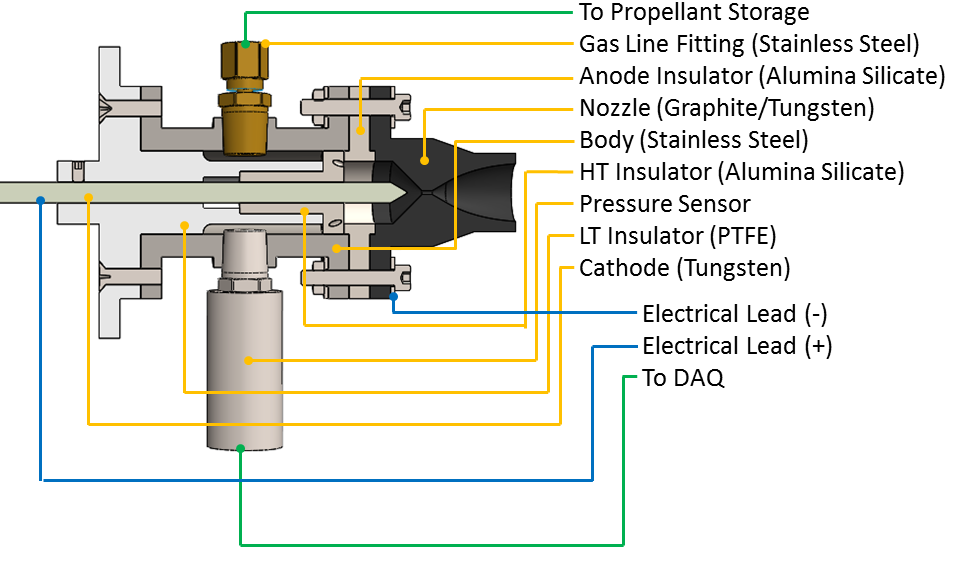
\includegraphics[width=\linewidth]{figs/cutaway_annotated.png}
  \caption[P17101 Arcjet Annotated Cutaway]{Components that are charged or exposed to extreme heat are electrically and thermally insulated. \textbf{Update with HV+ lead and remove tungsten material from nozzle.}
\label{fig:annotated-cutaway}
}
\end{figure}

\subsection{Power Conditioning Unit}
% Describe the inputs and desired outputs of the unit. Explain the theoretical justification behind the HV/HC approach. Describe the approach in theoretical terms and list practical limitations.
The electrical arc used to add energy to the gas is generated and sustained by the Power Conditioning Unit (PCU).
The PCU consists of separate high-voltage (HV) and high-current (HC) sides.
The HV side of the circuit initiates the arc, then the PCU switches to the HC ``side'' of the circuit to sustain a high-current arc.
This architecture is similar to a plasma torch and has been demonstrated in similar tabletop systems~\cite{park2015thesis}.

% explain HV side here
\SI{120}{\volt} AC power is supplied to the PCU from a standard wall outlet.
The HV side of the circuit raises the voltage by several orders of magnitude.
A tungsten rod serves as the cathode of the HV circuit, and the graphite nozzle of the thruster acts as the anode.  When the arc jumps between the cathode and anode across the flowpath, it closes the HC portion of the circuit.
This current passes through a coil that activates a reed switch, turning off the HV side of the PCU.\@

\begin{figure}[htp]
  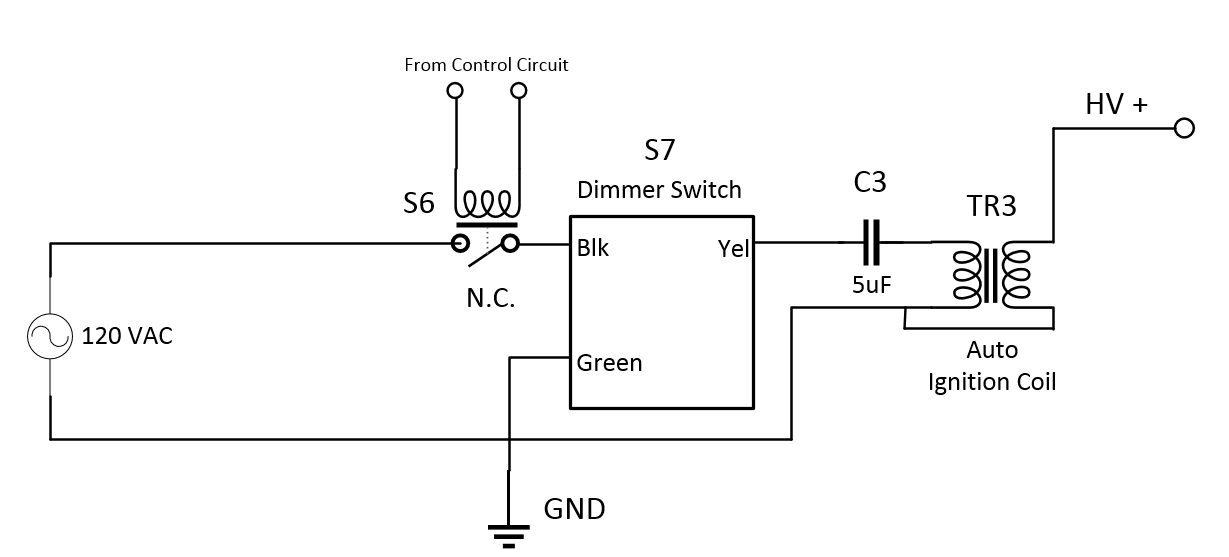
\includegraphics[width=\linewidth]{figs/hv-schematic.png}
  \caption{Wall AC power is converted to DC high voltage in order to initiate an arc.
\label{fig:hv-circuit}
}
\end{figure}

% explain HC side here
The HV side takes the 120 V AC input and passes it through a dimmer switch, resulting in a ``chopped'' AC wave.
A capacitor in series with the dimmer produces the derivative of the chopped AC wave, impulse functions.
This voltage is supplied to an automotive ignition coil, which returns the high voltage output that generates the arc across the anode and cathode.

\begin{figure}[htp]
  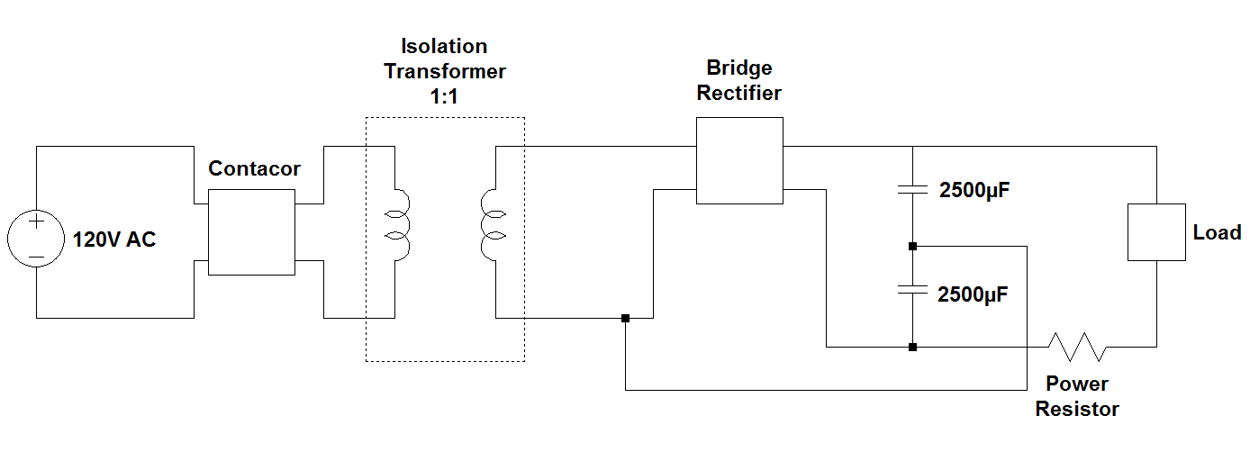
\includegraphics[width=\linewidth]{figs/hc-schematic.png}
  \caption{Anthony, please explain the high current circuit here.
\label{fig:hc-circuit}
}
\end{figure}

The HC circuit works by rectifying the \SI{120}{\volt} AC sine wave, resulting \SI{170}{\volt} DC.\@
The arc closes the circuit, allowing electrons to flow.
The high current comes from using small power resistors, which give a total resistance of \SI{30}{\ohm}.
The HC circuit has a coil that activates a reed switch when on.
The reed switch activates a relay which turns off the HV circuit.

During nominal operation, the PCU draws $900$--$1100$\si{\watt} from the wall outlet.

\subsection{Test Stand}
% Explain the physical apparatus that measures the system's outputs. Describe the interactions between the thruster and the test stand. Justify instrumentation selection.
The test stand is cantilevered in design, leveraging both the mass of the thruster and its operating thrust.
Because expected thrust output is low and load cells in that range are either very costly or lack the necessary accuracy this decision was made to allow the thruster mass to act as an offset that suits a more common range load cell.
The resolution of a 0--6\si{\kilo\gram} Omega LCAE-6kg load cell will capture this change in load reliably while also keeping equipment expenses reasonable.

The construction of the stand is largely 6061-T6 aluminum with the test platform assembled to an oil-impregnated bronze rod that allows for displacement vertically downwards on the load cell.
Two 6''$\times$8'' plates are welded at a right angle with a pair of gussets to form the main structure of the stand, and two bearing blocks are fastened several inches further up to capture the bronze bearing rod and test platform itself.
The thruster is mounted to the test platform using a set of three toe-clamps to make the set up and breakdown of the system simple and efficient.
The stand's construction allows for some variability in expected test results through a set of slots used to position the load cell. Since it offers a small form facto, the complete mechanical system can be accommodated in a range of different testing environments such as the engine test cell that is used to complete these initial studies.

Propellant is supplied by a gaseous nitrogen dewar at \SI{2200}{psi}.
The GN$_2$ is nominally regulated to \SI{20}{psi} before reaching a normally-closed solenoid valve.
GN$_2$ is flowed through the system for several seconds before PCU ignition to ensure only nitrogen is present in the thruster, and after PCU shutdown to cool hot hruster components.

\subsection{Data Acquisition \& Control}

Operation of the PCU and propellant solenoid as well as data acquisition (DAQ) is nominally controlled by a National Instruments MyDAQ device utilizing a LabVIEW Virtual Interface (VI).
Two DAQ devices were recognized as being readily available, the NI USB-6008 and the NI MyDAQ.\@
The USB-6008 device offers more overall channels (4 analog input) but with a much lower throughput (\SI{10}{kS/s}) and resolution (12-bit).
The MyDAQ device only offers 2 analog input channels but offers \SI{200}{kS/s} at 16-bit resolution. It was determined that the primary performance metric would be the thrust force generated during a burn with pressure inside the main body being a secondary performance metric.
Acquiring data for these metrics would only require two analog input channels and as such, the MyDAQ device was chosen for its superior precision.
Both devices were also capable of generating an output which would be sufficient to actuate the transistors, which in turn activate the PCU and propellant solenoid, so this parameter was not taken into consideration during device selection.

The test engineer starts and stops a test with the VI (see~\autoref{fig:VI-frontpanel}) from a computer connected to the test stand.
Once the proper channels are selected for both data acquisition (analog inputs) and system control (analog outputs), the DAQ parameters may be chosen (i.e.\ sample rate \& number of samples per channel).
The timing of solenoid and PCU events may also be adjusted via the front panel.
Once the VI is started, the solenoid and PCU will be activated respectively and DAQ will begin with a live readout being shown on the waveform chart displayed on the front panel.
When the VI is stopped, the user will be prompted to either save the data or to discard it.

\subsection{Safety Measures}
% Describe risk management in more detail. Consider ommitting this section~\cite{linden}.
In the event of a computer malfunction, an emergency shutoff button is wired into the circuit between the outlet and the PCU and the solenoid is normally closed and non-latching.
When a test is conducted, the test stand is placed in a well-ventilated Formula SAE engine test cell, and the control computer is located outside the testing room.
The VI monitors sensor data in real-time and shuts down operation when sensor parameters reach unsafe limits, and may be stopped via the stop button on the front panel or by the satisfaction of a number of safety interlocks present within the block diagram.
Examples of these interlocks are errors in the DAQ sequence, positive gauge pressure present in the thruster's main body before starting the VI, or a ten second timeout.

% Because of some charring observed in the plywood base during circuit operation, an informal test was performed on the power resistors under operational conditions to gain an estimate on the temperature changes over time.
% The graphs below show the average temperature increase is 7.4F per second. The charring temperature of wood is 250-300F, and a 10s burn would require a temperature buffer of 80-90F.
% In order to protect the wood enclosure a temperature cutoff was added to the power line that opens at 250F.

\section{Test Procedure}
% Describe the basic test plan in broad terms and how we approached testing. Describe the setup within the engine test cell and how the user interacts with the system.

\section{Results}
% Show results and how they compare to our predictions. Describe any failures and the problem solving process that occurred.

\section{Conclusions \& Recommendations}
% Evaluate the success of the project and make recommendations for improving it.

\section*{Acknowledgments}
The team thanks Mr.~Vincent Burolla for his unwavering support; the Mechanical Engineering Department, the Multidisciplinary Senior Design Department, and the Kate Gleason College of Engineering for their resources and workspaces; RIT Space Exploration and Boeing for sponsoring this project.

\bibliographystyle{IEEEtran}
\bibliography{p17101}


\onecolumn
\appendices{}
\counterwithin{figure}{section}
\section{PCU Schematic}
\begin{figure}[h!]
  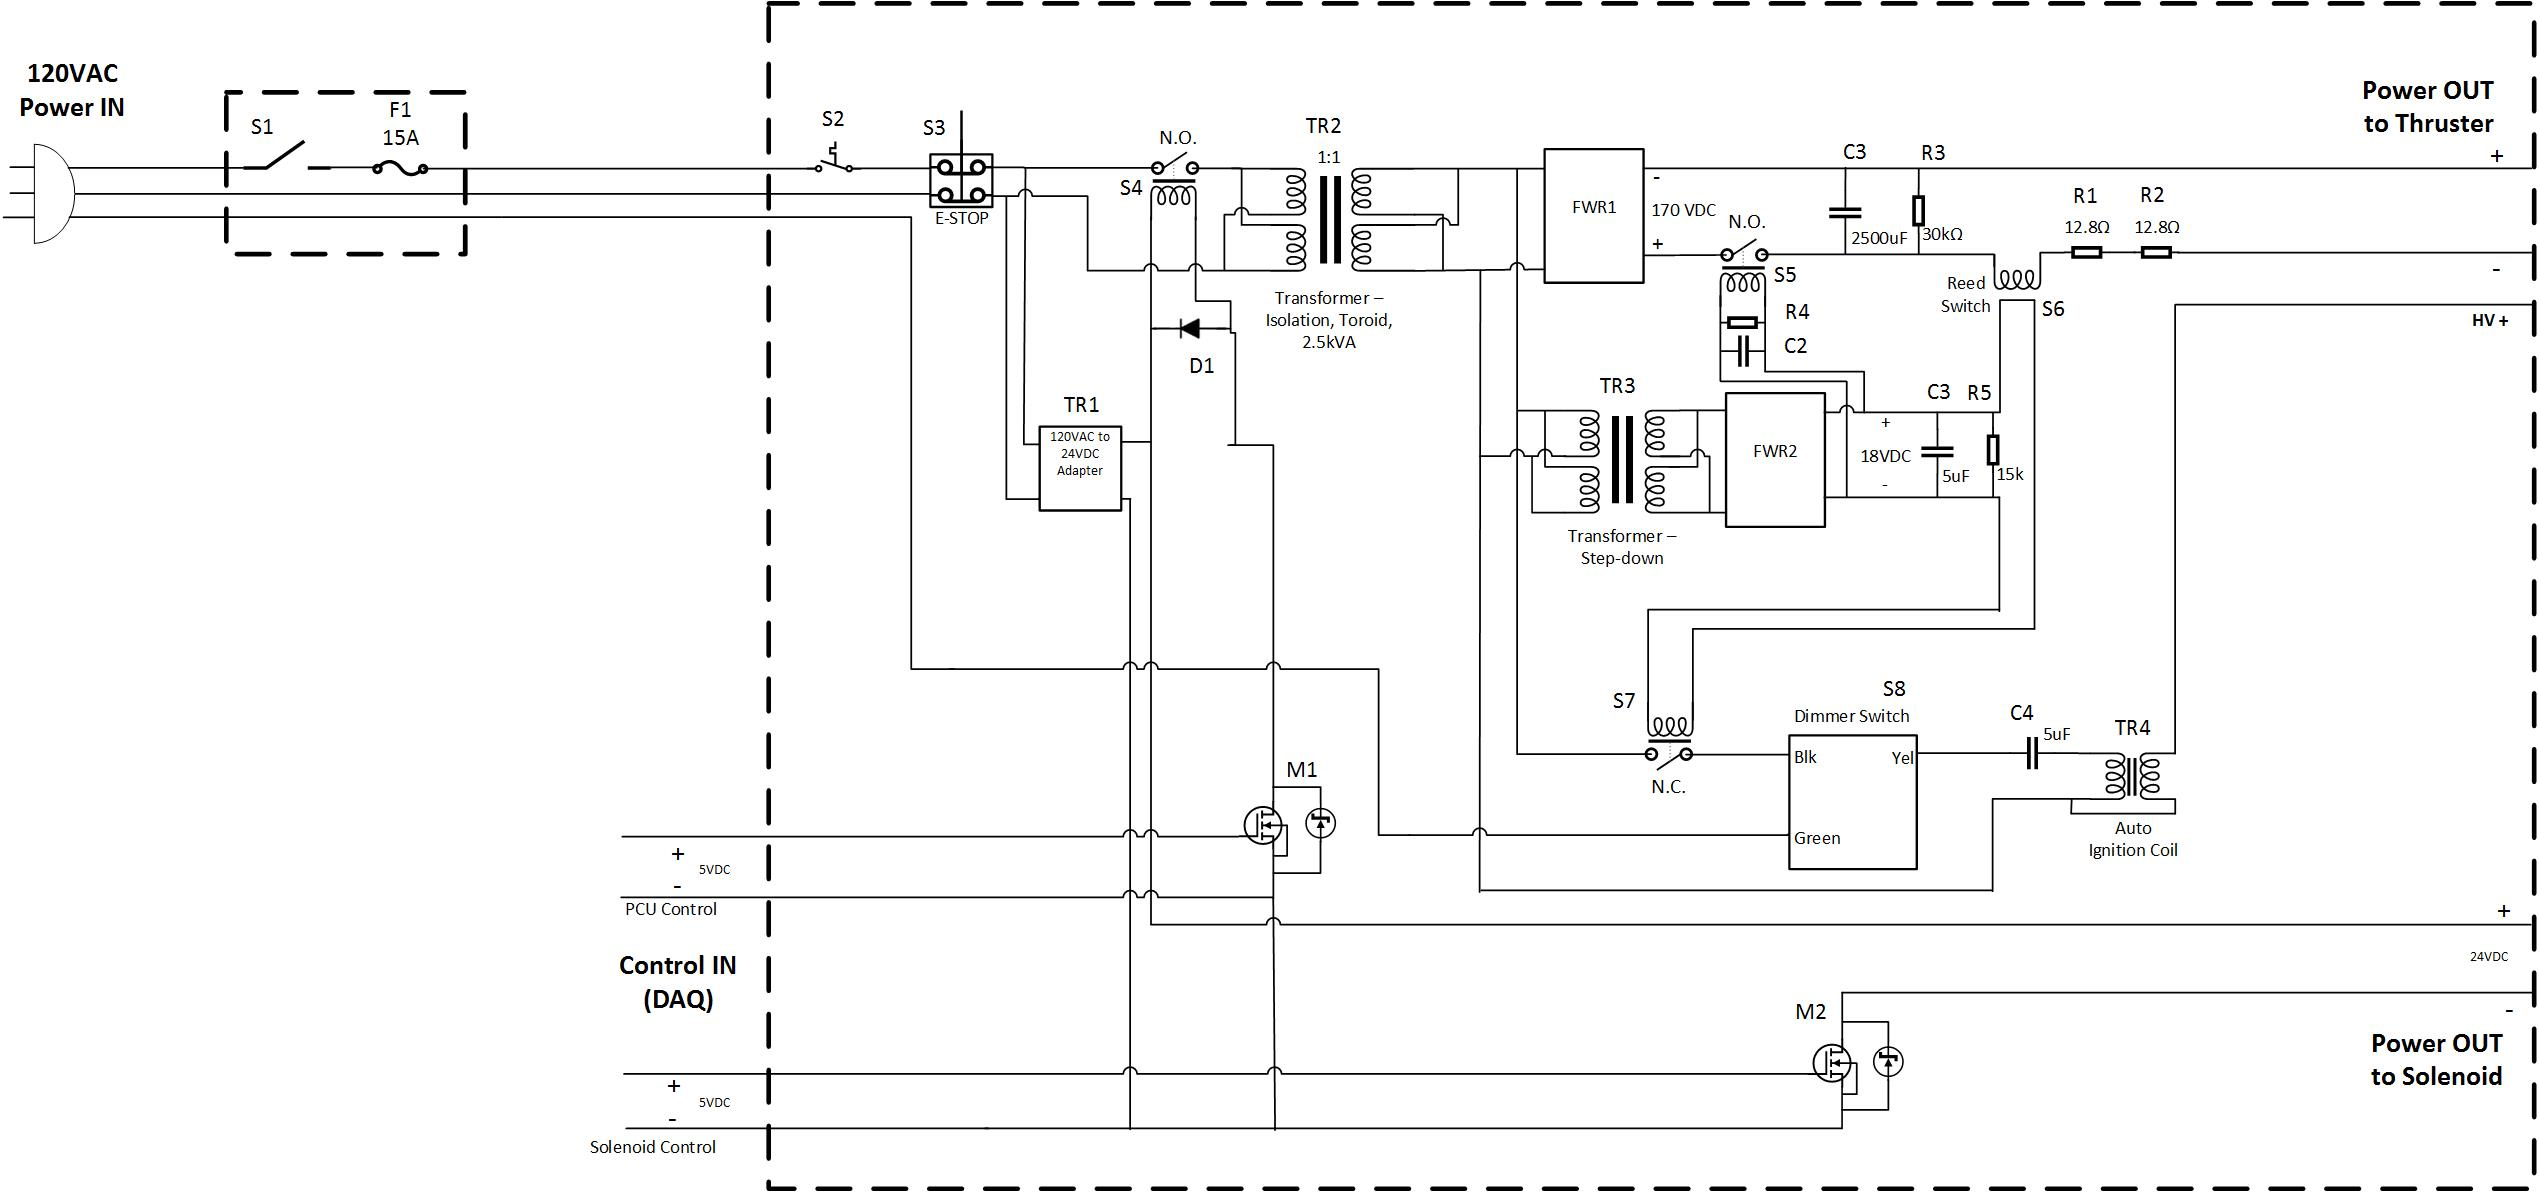
\includegraphics[angle=90,height=.9\vsize,keepaspectratio]{figs/PCU.jpg}
  \caption{Electrical diagram of the PCU.}
\label{fig:pcu-schematic}
\end{figure}

\section{Data Aqcuisition \& Control Virtual Interface}
% Images will need to be updated once proper data acquisition/recording and safety interlocks are implemented.
\begin{figure}[htp]
  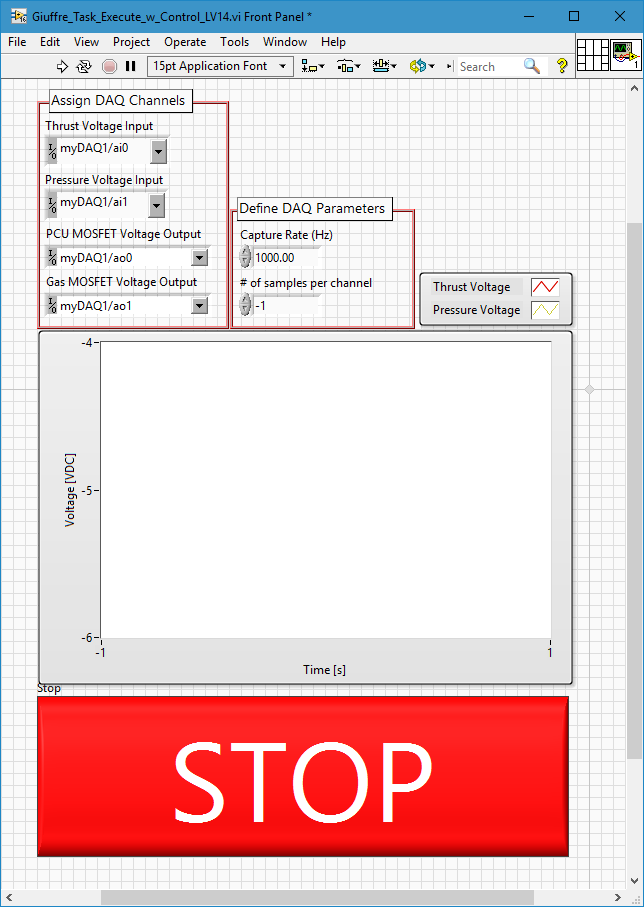
\includegraphics[height=.6\vsize,keepaspectratio]{figs/VI_30Mar17_FP.png}
  \caption{The user interface for the DAQ/Control VI.\@
\label{fig:VI-frontpanel}
}
\end{figure}

\begin{figure}[htp]
  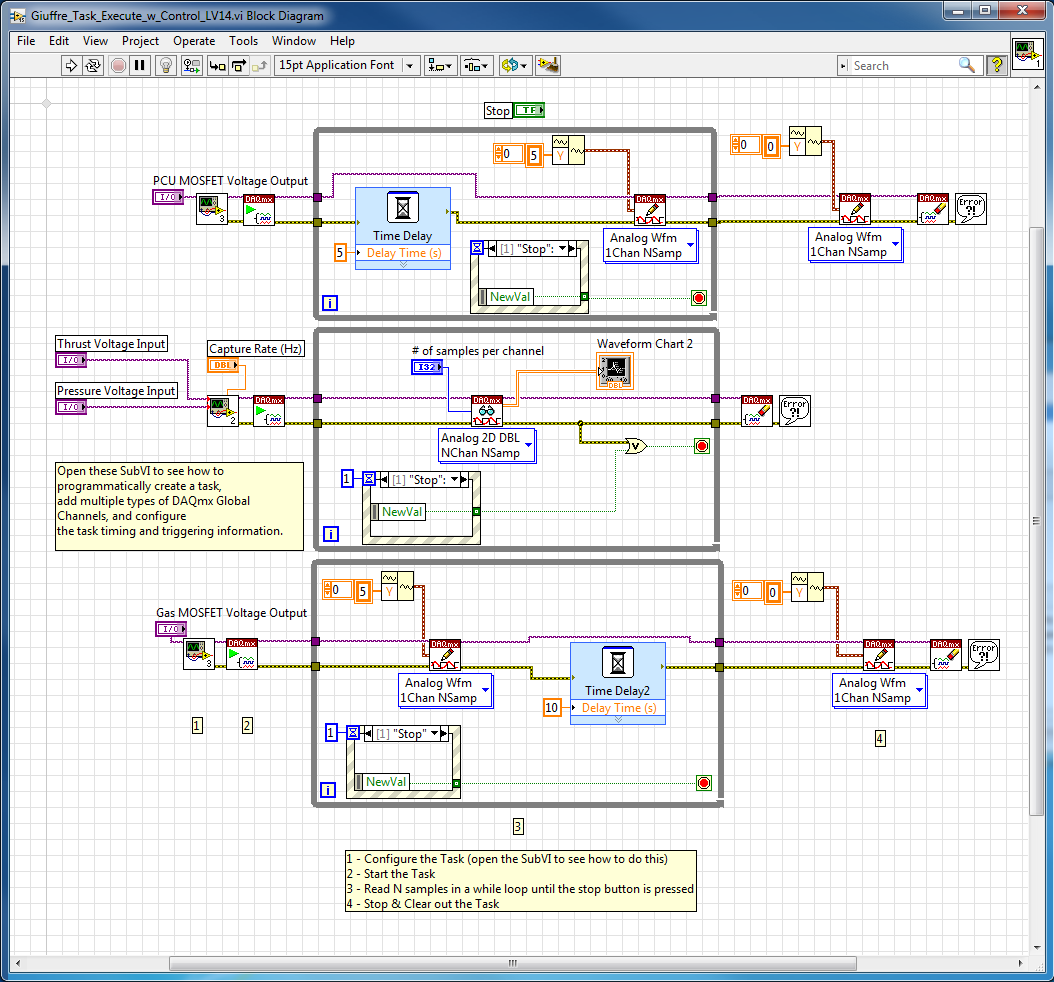
\includegraphics[height=.5\vsize,keepaspectratio]{figs/VI_30Mar17.png}
  \caption{The block diagram for the DAQ/Control VI.\@
\label{fig:VI-blockdiagram}
}
\end{figure}

\begin{figure}[htp]
  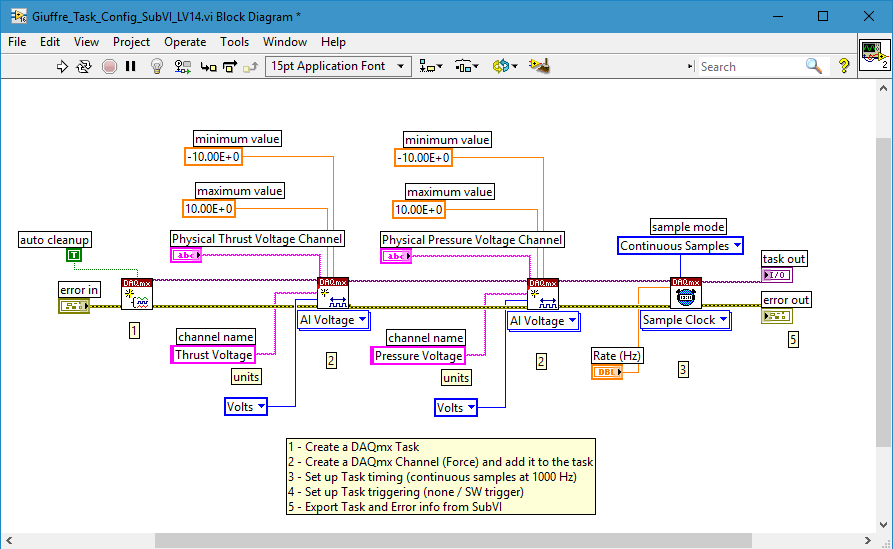
\includegraphics[height=.4\vsize,keepaspectratio]{figs/VI_30Mar17_SubVI.png}
  \caption{One of three sub-VIs used within the main VI to define channels \& tasks.
\label{fig:VI-subVI}
}
\end{figure}
\end{document}
